% Inverse CDF for the exponential(1): F(x)=1-exp(-x).
% U=1/2 maps exactly to X=ln 2.
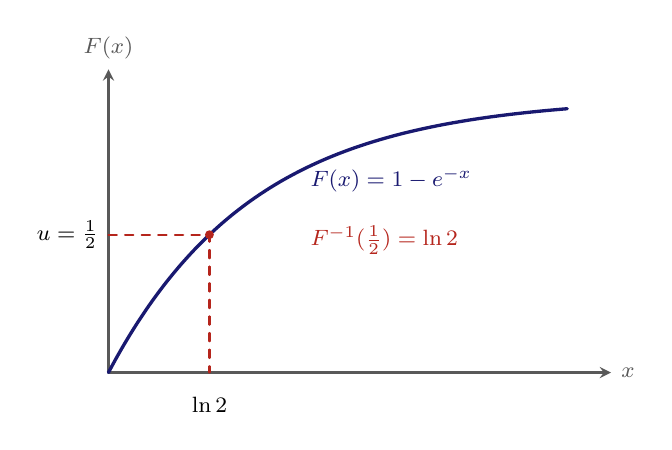
\begin{tikzpicture}[x=1.85cm,y=3.5cm,line cap=round,>=stealth]
  \draw[->,black!65,thick] (0,0)--(3.45,0) node[right,font=\footnotesize] {$x$};
  \draw[->,black!65,thick] (0,0)--(0,1.10) node[above,font=\footnotesize] {$F(x)$};
  \draw[MidnightBlue,very thick,domain=0:3.15,samples=65,smooth] plot (\x,{1-exp(-\x)});
  \draw[BrickRed,thick,dashed] (0,0.5)--(0.693147,0.5)--(0.693147,0);
  \fill[BrickRed] (0.693147,0.5) circle (1.6pt);
  \node[left,font=\footnotesize] at (0,0.5) {$u=\frac12$};
  \node[below,font=\footnotesize] at (0.693147,-0.055) {$\ln2$};
  \node[font=\footnotesize,anchor=west,text=MidnightBlue] at (1.32,0.7) {$F(x)=1-e^{-x}$};
  \node[font=\footnotesize,anchor=west,text=BrickRed] at (1.32,0.48) {$F^{-1}(\frac12)=\ln2$};
\end{tikzpicture}
